\documentclass{beamer}
\usepackage[T1]{fontenc}
\usepackage[utf8]{inputenc}
\usepackage{url}
\usepackage{ragged2e}
\usetheme{metropolis}
\setbeamercolor{background canvas}{bg=white}
\usepackage{tikz}
\usetikzlibrary{calc,arrows,positioning,shapes.geometric}
\usetikzlibrary{backgrounds}


\title{Writing with NAO}
\author{Adrien Bardes, Marius Dufraisse, Pierre Guetschel, Mengda Li}
%\institute{ENS Paris-Saclay}

\titlegraphic{\includegraphics[scale = 0.2]{logo.png}}
\begin{document}

\frame{\titlepage}

\begin{frame}{Goal of our project}
	\begin{itemize}
		\item We want to make our robot NAO write!
	\end{itemize}
	\begin{figure}[h]
		\centering
		\includegraphics[width = 0.8
		\linewidth]{NAO_writes.jpg}\cite{1}
	\end{figure}
\end{frame}


\begin{frame}{Methodology}
	%\tableofcontents
	\begin{figure}[h]
		\centering
		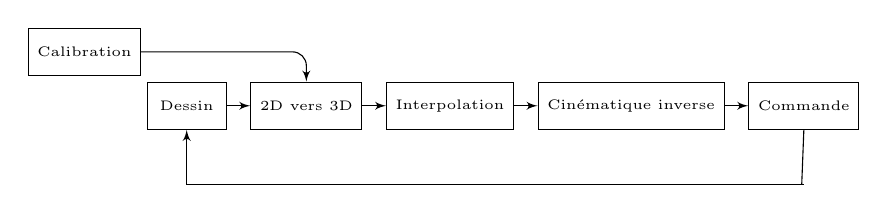
\begin{tikzpicture}[>=latex']
			\tikzset{block/.style= {draw, rectangle, align=center,minimum width=1cm,minimum height=6mm,font=\tiny},
			}
			\node [block]  (start) {Calibration};
			\node [block, below right = 1mm of start] (dess){Dessin};
			\node [block, right = 3mm of dess] (transfert){2D vers 3D};
			\node [block, right = 3mm of transfert] (interpolation){Interpolation};
			\node [block, right = 3mm of interpolation] (kin){Cinématique inverse};
			\node [block, right = 3mm of kin] (com){Commande};





			\path[draw, ->,rounded corners=5pt]
			(start) -| (transfert);

			\path[draw, ->]
			(dess) -- (transfert);
			\path[draw, ->]
			(transfert) -- (interpolation);
			\path[draw, ->]
			(interpolation) -- (kin);
			\path[draw, ->]
			(kin) -- (com);

			\coordinate (below scheme) at ($(com)!0.5!(interpolation)-(-2.22,1)$);
			\node[below =5mm of kin] (A){} ;
			\path[draw, ->] (com|-below scheme)-|(dess);
			\path[draw] (com.south)--(below scheme);

			%\node[below of=transfert](B){};
			%\path[draw, ->, rounded corners = 5pt]
			%(com) -- (A) -- (B) -- (dessin);
			%	(ADL) -- (AUL)
			%	(AUL) edge (A1)
			%	(A1) edge (A2)
			%	(A2) -- (AUR)
			%	(AUR) -- (ADR)
			%	(ADR) edge (AEnd)
			%
			%	(start) -- (BUL)
			%	(BUL) -- (BDL)
			%	(BDL) edge (B1)
			%	(B1) edge (B2)
			%	(B2) -- (BDR)
			%	(BDR) -- (BUR)
			%	(BUR) -- (BEnd);
		\end{tikzpicture}
	\end{figure}
\end{frame}

%\section{Analysis of handwriting and extraction of trajectory function}
%\begin{frame}{trajectory function}
%
%We formalize what we want to write by a trajectory function.
%\bigskip
%
%\includegraphics[scale = 0.3]{planning.jpg}\cite{2}
%\end{frame}
\section{Inverse kinematics}


\begin{frame}{Approching the goal trajectory}

	We approach this goal trajectory by solving a sequence of optimization problems: minimizing the errors between the goal trajectory and the real trajectory.
	\medskip

	\includegraphics[scale = 0.4]{tracking.jpg}\cite{2}
\end{frame}

\begin{frame}{An example of trajectory}
\begin{figure}
	\centering
	\includegraphics[width=0.8\linewidth]{path}
\end{figure}
\end{frame}

\begin{frame}{and its interpolation}
\begin{figure}
	\centering
	\includegraphics[width=0.8\linewidth]{x}
\end{figure}
\end{frame}

\subsection{Modeling the coordinate system}

\begin{frame}[allowframebreaks]{Modeling the coordinate system}

	\begin{columns}
		\begin{column}{0.5\textwidth}
			\justify
			The robot's arm is a 6-joint system.

			We find the position of end-effector (the pen) by composing a sequence of \emph{change of coordinates} matrix.
		\end{column}
		\begin{column}{0.5\textwidth}  %%<--- here
			\begin{center}
				\includegraphics[scale = 0.35]{arm.jpg}\cite{3}
			\end{center}
		\end{column}
	\end{columns}


	%\includegraphics[scale = 0.35]{coordinate.png}\cite{3}

	%\includegraphics[scale = 0.3]{joints.png}\cite{4}

	\center
	\includegraphics[scale = 1.8]{A-6R-manipulator-with-normal-configuration.png}\cite{4}

\end{frame}

\subsection{Finding the next ``angles step'' by computing the Jacobian}
\begin{frame}{Finding the next ``angles step'' by computing Jacobian i}


	\includegraphics[scale = 1.2]{slide_30.jpg}\cite{5}
\end{frame}

\begin{frame}{Finding the next ``angles step'' by computing the jacobian ii}

	\includegraphics[scale = 1.2]{slide_31.jpg}\cite{5}
\end{frame}

\begin{frame}{Finding the next ``angles step'' by computing the jacobian iii}

	\includegraphics[scale = 0.7]{eth1.PNG}\cite{6}
\end{frame}

\begin{frame}{Finding the next ``angles step'' by computing the jacobian iv}

	\includegraphics[scale = 0.3]{eth3.PNG}\cite{6}
\end{frame}

%     \includegraphics[scale = 0.2]{1_8N5jdpb0omhPkTHSzyIf5A.png}\cite{7}

\begin{frame}{Our results}
\begin{itemize}
\item With the previous trajectory.
\end{itemize}
\begin{figure}[h]
\centering
\includegraphics[width=0.8\linewidth]{elbowroll}
\end{figure}
\end{frame}

\begin{frame}{Influence of $\lambda$}
\begin{itemize}
	\item With the previous trajectory.
\end{itemize}
\begin{figure}[h]
	\centering
	\includegraphics[width=0.8\linewidth]{lambda}
\end{figure}
\end{frame}

\begin{frame}[allowframebreaks]{Bibliography}
	\begin{thebibliography}{9}

		\bibitem{1}
		NAO robot illustrating a TechCrunch article.
		\path{https://www.robotlab.com/blog/nao-robot-illustrating-a-techcrunch-article}

		\bibitem{2}
		Planification et suivi de trajectoires.
		\path{http://cas.ensmp.fr/~petit/smai/}

		\bibitem{3}
		\textit{Interfacing of Kinect Motion Sensor and NAO Humanoid Robot for Imitation Learning}.
		\path{https://www.youngscientistjournal.org/article/interfacing-of-kinect-motion-sensor-and-nao-humanoid-robot-for-imitation-learning}

		\bibitem{4}
		\textit{Formal Kinematic Analysis of a General 6R Manipulator Using the Screw Theory}

		\bibitem{5}
		Matt Boggus.
		\textit{Character Animation Forward and Inverse Kinematics}.
		\path{https://slideplayer.com/slide/12902351/}

		\bibitem{6}
		Marco Hutter, Roland Siegwart, and Thomas Stastny.
		\textit{Lecture «Robot Dynamics»: Summary}.
		\path{https://www.ethz.ch/content/dam/ethz/special-interest/mavt/robotics-n-intelligent-systems/rsl-dam/documents/RobotDynamics2017/14-summary.pdf}
		%\bibitem{7}
		%Luis Bermudez.
		%\textit{Overview of Jacobian IK}.
		%\path{https://medium.com/unity3danimation/overview-of-jacobian-ik-a33939639ab2}
		%\bibitem{y}
		%Emrehan Yavşan, Ayşegül Uçar.
		%\textit{Teaching human gestures to humanoid robots by using Kinect sensor}.
		%\path{https://www.researchgate.net/publication/282829504_Teaching_human_gestures_to_humanoid_robots_by_using_Kinect_sensor}
		%
		%\bibitem{x}
		%Oussama Khatib.
		%\textit{Springer Handbook of Robotics}.
	\end{thebibliography}
\end{frame}

\end{document}
